
\section{Motivation and Challenges}
\label{sec:motiv}
\vspace{-.2cm}	
	%\begin{figure}
	%	\centering
	%		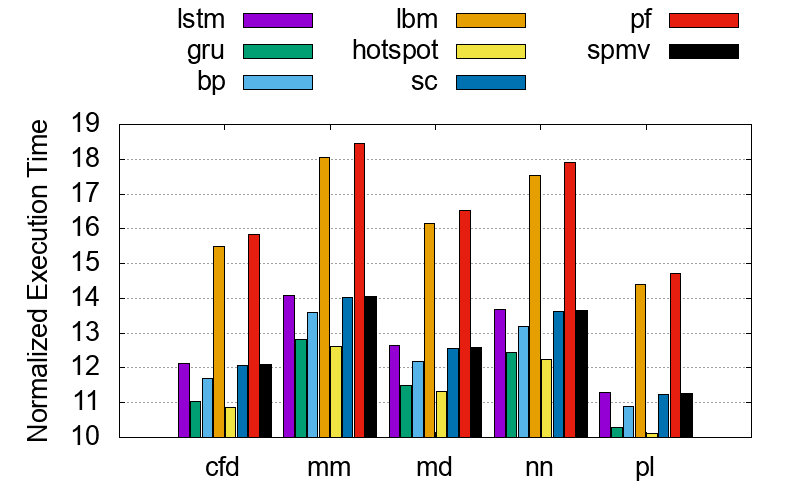
\includegraphics[width=8cm]{figures/seq_time.png}
	%	\caption{QoS violation for co-runs when the GPU is unpreemptable.}
	%	\label{fig:qos}
		%\vspace{-0.5cm}
	%\end{figure}
	
\subsection{QoS Issues of Non-Preemptable Kernels}
\label{sec:non-preemptable}
To understand the detrimental effect of non-preemptable kernel execution on QoS violation, we run 40 pairs of kernels (details in Section~\ref{sec:eval}) on an NVIDIA Volta GPU. Fig.~\ref{fig:qos} shows the performance degradation of the LC kernels when they are immediately launched after the BE kernels shown on the X axis.  Observe that QoS is violated for all the pairs even if the QoS target is as large as 10 times of the corresponding solo-run execution time when sharing is disabled. This is because the entire time the BE kernel is finishing normally, the LC kernel has to wait in queue, a clearly unacceptable solution.
%\nsout{Note that rescheduling kernels, 
%no matter how intelligent the algorithm is, cannot completely solve this problem.}{}
% 
%phenomena reflects the fact 
%It indicates that rescheduling strategy%, 
%no matter how intelligent the algorithm is, 
%cannot completely solve the problem of our concern.
%Since it is %\nsout{hard}{}
%already quite difficult, if not impossible, for us to predict the 
%arrival time of the LC kernels, launching a BE kernel without 
%any control on its resource usage may %\nsout{render 
%the whole GPU unusable for LC applications.}{}
%prevent LC applications from being executed because 
%all the resources have been claimed by the BE kernel. %According to the scheduling policy, LC applications 
%have to wait until the BE kernel is done. The QoS target is most likely violated in this case.
	
\subsection{Scalability Issues of Preemption-Based Solutions}
\begin{figure}
\vspace{-0.4in}
		\centering
		\begin{minipage}{0.45\linewidth}
		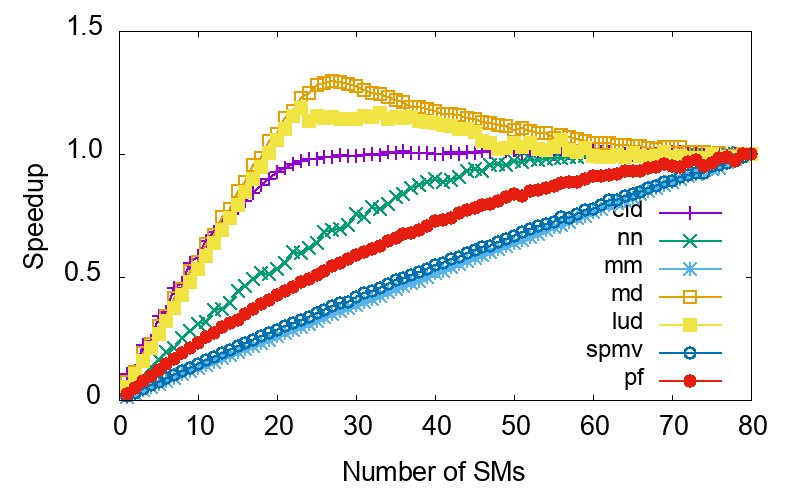
\includegraphics[width=\linewidth]{figures/solo_scalability/sm_scale_new.png}
		%\vspace{-0.2cm}
		\caption{Solo-run scalability with respect to the number of SMs}
		\label{fig:solo-sm}
		\vspace{-0.5cm}
	\end{minipage}
	\hfill
	\begin{minipage}{0.45\linewidth}
		\centering
		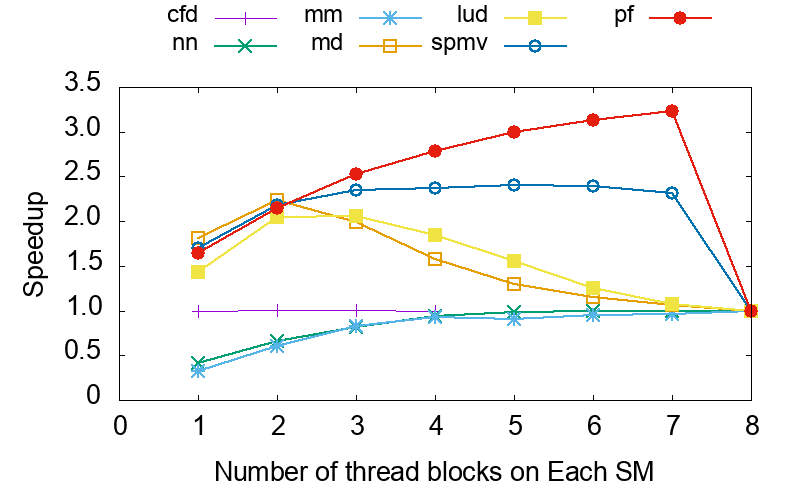
\includegraphics[width=\linewidth]{figures/solo_scalability/blk_scale_mul.png}
		%\vspace{-0.2cm}
		\caption{Solo-run scalability with respect to the number of thread blocks on each SM}
		\label{fig:solo-bl}
		\vspace{-0.5cm}
	\end{minipage}
	\end{figure}
	%\vspace{-0.8cm}
Recent work, such as FLEP~\cite{Wu:ASPLOS2017} and Effisha~\cite{Chen:PPoPP2017}, has proposed low-overhead software-based mechanisms to  realize preemption on GPUs.  With the capability of preemption, we can easily address the QoS issue by preempting  the BE kernel whenever an LC arrives. However, the drawback of preemption is that LC kernels monopolize all the available resources regardless of how efficiently it will utilize them. We show the scalability of 7 benchmarks in Fig. \ref{fig:solo-sm} and Fig.~\ref{fig:solo-bl} when we respectively increase the number of SMs and the number of thread blocks within each SM. Since the default scheduling uses up the SMs and thread blocks, the results show that less resource does not necessarily lead to worse performance. Moreover, different applications may have different scaling characteristics. For example, MM (matrix multiplication) prefers more computational resources, while MD's performance culminates with a small portion of the resources (i.e., 26 SMs or 2 thread blocks per SM).

% Figure \ref{fig:solo-sm} shows speedups of different applications with
% the number of SMs where there are 8 (4) TBs are scheduled on each SM and figure 
% \ref{fig:solo-bl} is scalabilities of the number of TBs on each SM. The size of 
% a TB is 256. Note all the kernels are able to run 8 TBs on an SM except CFD because each CFD thread uses 52 registers. 
%The idea of SM-centric transformation ~\cite{Wu+:ICS15} is adopted to show scalabilities of the kernels (details in Section~\ref{sec:system}).
%The benefit is that we have the ability of fine tuning the thread blocks being yielded to an LC kernel. We are able to
%control how many SMs to use and how many thread blocks to run on each used SM by an LC 
%application.
% These two figures tell us the following important things regarding to resource allocation.
%\begin{enumerate}
%\item 
% First, less resources could have positive speedup, that is, more resources don't guarantee better performance. %In Figure \ref{fig:solo-sm}, the performance of MD
%and LUD is linearly proportional to the amount of resources when the number of SM is less than 20. The speedup will be larger than 1 around 23 SMs and then the performance will start to decrease as 
%more resources are given to the applications. The same phenomena occurs in the scalabilities with respect to the number of TBs on each SM as well. 
%\item 
% Second, the performance could be saturated when partial resources are allocated. %This fact is reflected by the CFD and NN in Figure \ref{fig:solo-sm} 
% %and by NN and MM in Figure \ref{fig:solo-bl}. The CFD kernel's performance is saturated when 20 SMs are allocated, while NN saturates around 50 SMs. 
% %\item 
% Third, given the same amount resources, the performance of an application could have significant difference for different configurations. 
%       %Take the PF application as an example. Assume that
% %the application is given a half of the resources. The configuration (40, 8) will have speedup less than 1 while the configuration (80, 4) provides more than 2X speedup. 
% Our notation is that
% the first component of the configuration tuple is the number of SM being used and the second one is the TBs on those SMs.
% %\item 
% Fourth, the scalability is case dependent. %Obviously, it could be super-linear, linear and sub-linear based upon the observation on all 
% %the curves in two figures.
% %\item 
% Fifth, the hardware is generally underutilized. %An application could possibly oversubscribe resources if it runs alone on a GPU. The oversubscribing provides either 
      %no speedup or slowdown. The excessive resources could be freed up for better hardware utilization without hurting applications' performance. 
%\end{enumerate}
%}

	%\begin{figure*}
	%	\centering
	%	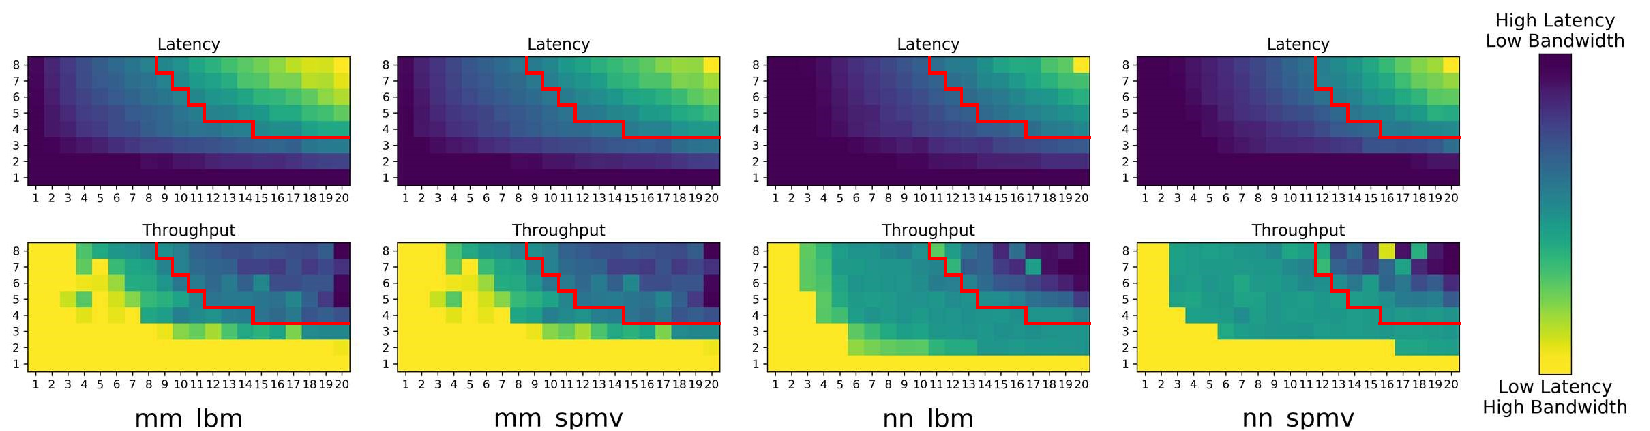
\includegraphics[width=\textwidth]{figures/corun_scalability_cropped.pdf}
	%	%\vspace{-0.5cm}
	%	\caption{Co-Run Scalability}
	%	\label{fig:corun-scalability}
	%	%\vspace{-0.15cm}
	%\end{figure*}
	\subsection{Spatial Co-Running and its Challenges}
%The rescheduling approach and the preemption-based approach are just two extreme points in a rich 
%design space of GPU spatial sharing among co-running applications. 
In order to run a pair of BE and LC application simultaneously, we need a mechanism for the BE application to be able to yield resources (entire SMs or thread block slots of SMs) to the LC application. Though the reduced resource availability and introduced contention cause slowdown for both kernels, we observe such a mechanism allows one to produce a better trade-off between QoS guarantees and overall GPU utilization. 
%We care about only the slowdown of the LC kernel and the overall throughput of the co-run pair.
%Therefore, 
% Such a mechanism allows one 
% to produce a better trade-off between QoS guarantees and overall GPU utilization. This leaves the following goals for this paper: \\
% %\begin{itemize}
% 	1. Better saturate GPU resources by spatially co-running two kernels rather than one.
% 	\\
% 	2. Keep the run time of the Latency Critical (LC) kernel under its QoS deadline \\
% 	3. Maximize the overall throughput of a BE-LC pair subject to latency constraint  %\end{itemize}
		%In order to combat poor resource utilization in GPUs, we suggest that a finer-grained sharing approach is required. Even when a whole GPU is occupied with thread blocks, it is not necessarily being maximally utilized, as suggested by the performance saturation shown in Figures \ref{fig:solo-sm} and \ref{fig:solo-bl}. Combating this is especially important at the datacenter scale where poor resource utilization drives up costs for GPU usage costs massively. Idle GPUs which only run QoS sensitive tasks and sit idle in between exacerbate this problem further. Running thread blocks from two kernels in a spatially-shared environment should make better use of some underutilized resources and make a more dynamic allocation methodology possible. This section will consider the differences between solo-run and co-run scalability to explore feasibility.
		%\par Unless a kernel manages to fully utilize on all shared resources simultaneously, there is potentially an opportunity to better utilize all the available hardware.
		%\par In order to combat poor resource utilization in GPUs, we can transform the BE application to yield resources for the co-running LC application. Consequently the kernels interfere with each other causing performance degradation. 
		
	\begin{figure*}%[h]
	\vspace{-0.5cm}
		\centering
		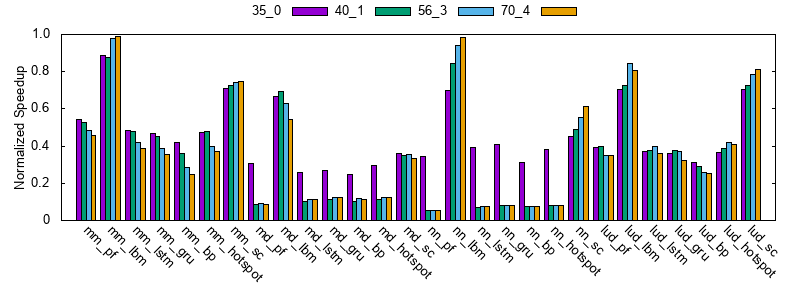
\includegraphics[width=\textwidth,height=3cm]{figures/mot_qperf.png}
		%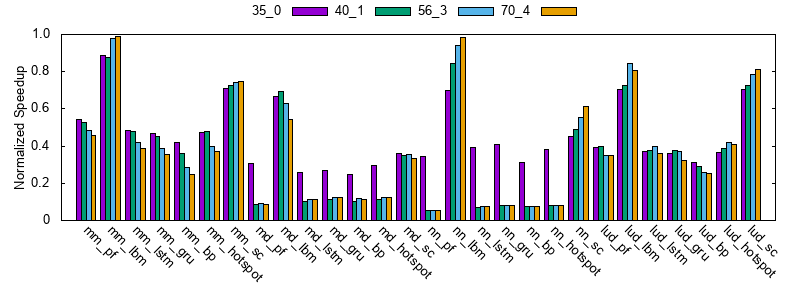
\includegraphics[width=9cm]{figures/mot_qperf.png}
		%\vspace{-0.2cm}
		\caption{LC kernel speedup with 280 thread blocks being allocated}
		\label{fig:corun_perf}
		\vspace{-0.5cm}
	\end{figure*}
To understand the complexity of the interference due to co-running, we run 40 kernel pairs with $280$ thread blocks allocated to each of the LC kernels. Fig. \ref{fig:corun_perf} shows the performance degradation of the LC kernels with four different configurations. On the X axis, the notation $A$\_$B$ represents a BE kernel $A$ co-running with a LC kernel $B$. Observe that the slowdown varies significantly across LC kernels or even the co-runs of the same LC kernel with different BE kernels. Fig.~\ref{fig:corun_thrpt} reports the overall throughput improvement (defined in Section~\ref{sec:eval}) and demonstrates the difficulty of predicting the best configuration for the co-runs.

% and \ref{fig:corun_thrpt}. 
% The notation used in the paper is the following. %The first component in the co-run pair is BE application, while the second is LC kernel. 
% The first number and the second one in SM configuration is the number of SM being yield to LC kernel and the number of TBs on these SMs, respectively. These two 
% figures shows that different pairs have different preference toward resource allocation. The resource allocation becomes even more complicated when the 
% QoS and throughput are taken into account. %For example at 5X QoS , the pair MM\_BP prefer inter-SM sharing from both QoS and throughput perspectives while the pair vote for the configuration 40\_1 and 
%NN\_LBM favors intra-SM 70\_4 sharing for both QoS and throughput. MM\_GRU likes intra-SM for throughput but inter-SM for QoS performance. Note that there is nothing special
%for $280$ TBs for LC kernel. %The same phenomena could be observed for difference total number of TBs. %The rule of thumb is that this number 
%should have as many as possible divisors between 1 and 8 to see such difference. 
%Therefore, 
% Different pair prefers different resource allocation to maximize
% the throughput even if the QoS is satisfied. %This is the focus of our paper.
%To understand the complexity of the interference due to spatial co-run\nsout{ning}{}, 
%we use MM and NN as BE applications and SPMV and LBM as LC applications, 
%and co-run each BE-LC application pair. For simplicity, we allow the BE application 
%to yield an arbitrary subset of SMs and the same number of thread blocks on each of those SMs. 
%Since the GPU has \nsout{20}{80} SMs and each SM can \nsout{run}{accommodate} up to 8 thread blocks due to the hardware limit, 
%each co-run pair has \nsout{160}{640} configurations for spatial sharing. Figure~\ref{fig:corun-scalability} 
%shows the performance degradation of the co-running applications. 
%In each column, the top figure shows the performance degradation for the LC application 
%and the bottom for the BE application. The top-right corner of each figure indicates 
%that the BE application yields the whole GPU to the LC application, maximizing QoS, 
%but providing no throughput to itself. Darker color means worse LC performance, 
%but higher BE throughput. The overall trend is clear and intuitive: 
%Yielding more resource improves the performance of the LC application but degrades the performance of the BE application.
\vspace{-0.7cm}
	\begin{figure*}[h]
		\centering
		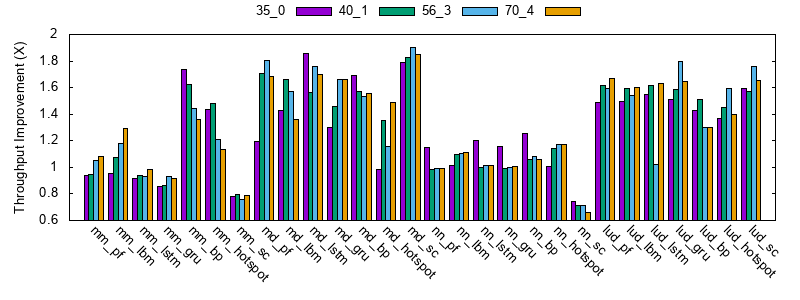
\includegraphics[width=\textwidth,height=3cm]{figures/mov_thrpt.png}
		%\includegraphics[width=9cm]{figures/mot_thrpt.png}
		%\vspace{-0.2cm}
		\caption{Overall throughput improvement}
		\label{fig:corun_thrpt}
		\vspace{-1.3cm}
	\end{figure*}
%From the boundary represented by the red curve to the top-right corner, 
%we have all the configurations that can satisfy the QoS requirement of the LC application. 
%Ideally, we should chose a configuration (very possibly on the boundary) in this region 
%which leads to minimum performance degradation for the BE application. 
%A naive online brute-force approach that tries all possible configurations and 
%chooses the optimal configuration would take too long and significantly violates QoS in the process.  
%For example, for the nn and spmv kernel co-run, 135 of the 160 runs violate QoS. 
%Unfortunately, the substantial differences between kernel behavior with and without 
%contention means the solo-run data is not very helpful for prediction. 
%The problem is especially challenging based on how different the degradation patterns 
%can be for different co-runs. For instance, co-runs involving the NN kernel experience
%much faster degradation of the QoS performance with fewer SMs than co-runs with MM. 
%Further, while a seemingly plausible solution is to profile all co-run configurations 
%offline to find the optimal configuration, it is not practical 
%because the applications may not be available offline, especially in a data center setting 
%where users may submit arbitrary applications. 
% In summary, to achieve the goals, this paper addresses the following challenges:
% %\begin{itemize}
% 	%\item 
%  estimating the co-running performance of kernels without extensive benchmarking,
% 	%\item 
% searching for the configuration whose throughput is maximized QoS is satisfied and %among many possible configurations for maximum throughput among those that satisfy QoS \\ %\item 
% 	minimizing the time taken to complete the configuration search
%\end{itemize}